% Data: completed presentation/FIXED_I_BY_H_CONTRASTS.csv and
% CHECKER_MODERATION_CONTRASTS.csv; primary frame, horizon 16.
% Independently checked in INTERACTION_TABLE_CHECK.json.
\begin{figure}[t]
\centering
\begingroup
\definecolor{resultblue}{HTML}{0072B2}
\definecolor{resultorange}{HTML}{D55E00}
\newcommand{\resultheatcell}[3]{%
  \pgfmathtruncatemacro{\shadepct}{5+5*abs(#3)}
  \ifnum#3<0
    \filldraw[fill=resultorange!\shadepct,draw=black!20]
      (#1,{#2-0.43}) rectangle ({#1+1.15},{#2+0.43});
  \else\ifnum#3>0
    \filldraw[fill=resultblue!\shadepct,draw=black!20]
      (#1,{#2-0.43}) rectangle ({#1+1.15},{#2+0.43});
  \else
    \filldraw[fill=black!3,draw=black!20]
      (#1,{#2-0.43}) rectangle ({#1+1.15},{#2+0.43});
  \fi\fi
  \ifnum#3>0
    \node at ({#1+0.575},#2) {$+#3$};
  \else
    \node at ({#1+0.575},#2) {$#3$};
  \fi
}
\newcommand{\resultheatrow}[8]{%
  \node at (0,-#1) {#2};
  \node at (1.3,-#1) {#3};
  \node at (2.4,-#1) {#4};
  \node at (3.5,-#1) {#5};
  \resultheatcell{4.35}{-#1}{#6}
  \resultheatcell{5.7}{-#1}{#7}
  \resultheatcell{7.05}{-#1}{#8}
}
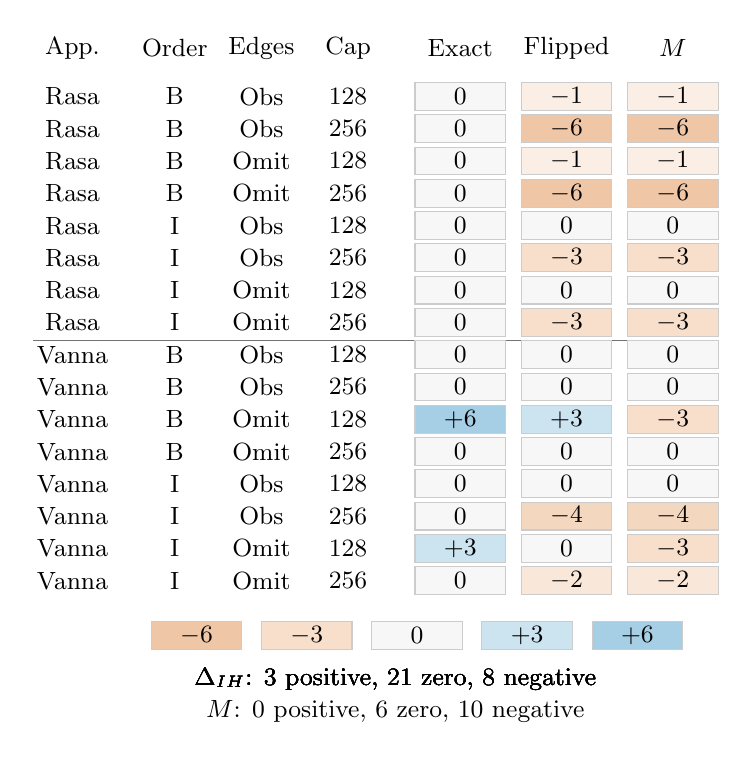
\begin{tikzpicture}[x=1cm,y=0.41cm,font=\small]
  \node at (0,0.5) {App.};
  \node at (1.3,0.5) {Order};
  \node at (2.4,0.5) {Edges};
  \node at (3.5,0.5) {Cap};
  \node at (4.925,0.5) {Exact};
  \node at (6.275,0.5) {Flipped};
  \node at (7.625,0.5) {$M$};
  \resultheatrow{1}{Rasa}{B}{Obs}{128}{0}{-1}{-1}
  \resultheatrow{2}{Rasa}{B}{Obs}{256}{0}{-6}{-6}
  \resultheatrow{3}{Rasa}{B}{Omit}{128}{0}{-1}{-1}
  \resultheatrow{4}{Rasa}{B}{Omit}{256}{0}{-6}{-6}
  \resultheatrow{5}{Rasa}{I}{Obs}{128}{0}{0}{0}
  \resultheatrow{6}{Rasa}{I}{Obs}{256}{0}{-3}{-3}
  \resultheatrow{7}{Rasa}{I}{Omit}{128}{0}{0}{0}
  \resultheatrow{8}{Rasa}{I}{Omit}{256}{0}{-3}{-3}
  \draw[black!55] (-0.5,-8.55) -- (8.2,-8.55);
  \resultheatrow{9}{Vanna}{B}{Obs}{128}{0}{0}{0}
  \resultheatrow{10}{Vanna}{B}{Obs}{256}{0}{0}{0}
  \resultheatrow{11}{Vanna}{B}{Omit}{128}{6}{3}{-3}
  \resultheatrow{12}{Vanna}{B}{Omit}{256}{0}{0}{0}
  \resultheatrow{13}{Vanna}{I}{Obs}{128}{0}{0}{0}
  \resultheatrow{14}{Vanna}{I}{Obs}{256}{0}{-4}{-4}
  \resultheatrow{15}{Vanna}{I}{Omit}{128}{3}{0}{-3}
  \resultheatrow{16}{Vanna}{I}{Omit}{256}{0}{-2}{-2}
  \foreach \x/\value in {1.0/-6,2.4/-3,3.8/0,5.2/3,6.6/6}
    \resultheatcell{\x}{-17.7}{\value}
  \node at (4.1,-19.05) {$\Delta_{IH}$: 3 positive, 21 zero, 8 negative};
  \node at (4.1,-20.05) {$M$: 0 positive, 6 zero, 10 negative};
\end{tikzpicture}
\endgroup
\caption{Complete primary impact--history interaction frame, centered on zero.
Exact and Flipped contain the 32 contrasts
$\Delta_{IH}=D(IH)-D(I)-D(H)+D(C)$; the third column is
$M=\Delta_{IH}^{\mathrm{flip}}-\Delta_{IH}^{\mathrm{exact}}$.
B/I denote blocked/interleaved order, Obs/Omit denote observed/omitted edges,
and Cap is the native task-request ceiling. Blue denotes positive values, orange negative
values; signed numbers retain the interpretation without color. Each arm has
48 repeated reference opportunities across three recorded passes. Flips use
the known seeded mask-generation probability 0.25, which is neither a
significance-test value nor an estimated natural checker-error rate. Zero
interaction does not establish mechanism independence, and negative interaction
does not require IH to perform worse than an individual arm.}
\Description{Sixteen rows pair exact and flipped judgment conditions and show
their difference. All eight Rasa exact contrasts are zero; its flipped values
are minus 1, minus 6, minus 1, minus 6, zero, minus 3, zero, minus 3 in
blocked then interleaved order, observed then omitted edges, and ascending
128/256 ceilings. Vanna exact contrasts are zero except plus 6 for blocked
omitted 128 and plus 3 for interleaved omitted 128. Vanna flipped contrasts
are zero except plus 3 for blocked omitted 128, minus 4 for interleaved
observed 256 and minus 2 for interleaved omitted 256. Across 32 interactions
there are 3 positive, 21 zero and 8 negative values. All 16 moderation values
are zero or negative: 6 zero and 10 negative.}
\label{fig:result-interactions}
\end{figure}
